% Generated by hw1/main.cpp -- do not edit by hand.
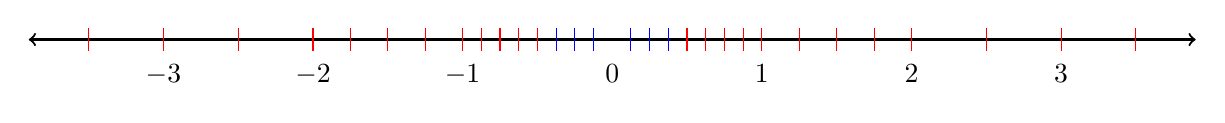
\begin{tikzpicture}[xscale=1.9, yscale=0.8]
  \draw[thick,<->] (-3.9,0) -- (3.9,0);
  % elements of F
  \draw[red] (0.5,0.18) -- (0.5,-0.18);
  \draw[red] (-0.5,0.18) -- (-0.5,-0.18);
  \draw[red] (0.625,0.18) -- (0.625,-0.18);
  \draw[red] (-0.625,0.18) -- (-0.625,-0.18);
  \draw[red] (0.75,0.18) -- (0.75,-0.18);
  \draw[red] (-0.75,0.18) -- (-0.75,-0.18);
  \draw[red] (0.875,0.18) -- (0.875,-0.18);
  \draw[red] (-0.875,0.18) -- (-0.875,-0.18);
  \draw[red] (1,0.18) -- (1,-0.18);
  \draw[red] (-1,0.18) -- (-1,-0.18);
  \draw[red] (1.25,0.18) -- (1.25,-0.18);
  \draw[red] (-1.25,0.18) -- (-1.25,-0.18);
  \draw[red] (1.5,0.18) -- (1.5,-0.18);
  \draw[red] (-1.5,0.18) -- (-1.5,-0.18);
  \draw[red] (1.75,0.18) -- (1.75,-0.18);
  \draw[red] (-1.75,0.18) -- (-1.75,-0.18);
  \draw[red] (2,0.18) -- (2,-0.18);
  \draw[red] (-2,0.18) -- (-2,-0.18);
  \draw[red] (2.5,0.18) -- (2.5,-0.18);
  \draw[red] (-2.5,0.18) -- (-2.5,-0.18);
  \draw[red] (3,0.18) -- (3,-0.18);
  \draw[red] (-3,0.18) -- (-3,-0.18);
  \draw[red] (3.5,0.18) -- (3.5,-0.18);
  \draw[red] (-3.5,0.18) -- (-3.5,-0.18);
  % subnormal numbers (Definition 1.15)
  \draw[blue] (0.125,0.18) -- (0.125,-0.18);
  \draw[blue] (-0.125,0.18) -- (-0.125,-0.18);
  \draw[blue] (0.25,0.18) -- (0.25,-0.18);
  \draw[blue] (-0.25,0.18) -- (-0.25,-0.18);
  \draw[blue] (0.375,0.18) -- (0.375,-0.18);
  \draw[blue] (-0.375,0.18) -- (-0.375,-0.18);
  % axis labels
  \node[below] at (-3,-0.25) {$-3$};
  \node[below] at (-2,-0.25) {$-2$};
  \node[below] at (-1,-0.25) {$-1$};
  \node[below] at (0,-0.25) {$0$};
  \node[below] at (1,-0.25) {$1$};
  \node[below] at (2,-0.25) {$2$};
  \node[below] at (3,-0.25) {$3$};
\end{tikzpicture}
